%\documentclass{cumcmthesis}
\documentclass[withoutpreface,bwprint]{cumcmthesis} %去掉封面与编号页,电子版提交的时候使用。


\usepackage[framemethod=TikZ]{mdframed}
\usepackage{url}   % 网页链接
\usepackage{subcaption} % 子标题
\usepackage{fancyhdr} 
\usepackage{color}
\usepackage{diagbox}
\usepackage{longtable,booktabs}
\usepackage{setspace}
\usepackage{pythonhighlight}


\title{题目}
\tihao{C}
\supervisor{ }
\yearinput{2022}
\monthinput{08}
\dayinput{05}

\begin{document}
	
	\maketitle
	\begin{abstract}
		摘要
		
		
		\quad
		
		
		\keywords{关\quad  键\quad  字\quad }
\end{abstract}

%\begin{spacing}{1.25}
%	\tableofcontents
%\end{spacing}   

\setcounter{page}{1}    

\section{问题重述与问题分析}
\subsection{问题重述}
玻璃是早期丝绸之路的重要商品,从西亚和埃及地区传入我国后, 古人因地制宜、就地取材制作出外观相似但化学成分不同的玻璃制品。玻璃炼制时需要助熔剂, 不同的助熔剂会导致玻璃的化学成分不同,例如铅钡玻璃和钾玻璃分别以铅矿石和草木灰作为助熔剂。同时, 古代玻璃易与外界环境进行元素交换而导致化学成分比例发生改变。


现有提供高钾玻璃和铅钡玻璃的相关数据,完成下列问题:


\begin{enumerate}
	\item 分析玻璃文物表面风化和玻璃类型、纹饰和颜色的关系;对不同的玻璃类型分析表面风化与否和玻璃化学成分含量之间的统计规律;根据风化点的检测数据预测风化前的化学成分含量;
	\item 根据附件数据分析铅钡玻璃和高钾玻璃的分类规律;对不同的玻璃类型,选择适当的化学成分划分亚类,并给出具体 的方法和结果,并对分类结果进行合理性和敏感性分析;
	\item 针对附件表单3的化学成分,鉴别其所属的类型,同样需要对结果进行敏感性分析;
	\item 分析不同类别玻璃文物的化学成分之间的关系以及比较不同类别化学成分关系的差异性。
\end{enumerate}


\subsection{问题分析}

\subsubsection{数据预处理}

\subsubsection{问题一的分析}

问题一要求分析附件表单1中文物表面风化与玻璃类型、颜色和纹饰之间的关系,随后分析表单2数据, 得出风化与化学成分含量的统计规律,最后依据表单2风化点的检测数据,预测风化前的化学成分含量。 本文首先对附件表单1的数据进行可视化, 作出以玻璃类型、纹饰和颜色为自变量,是否风化为因变量的三维气泡图,再对高钾玻璃和铅钡玻璃分别作风化 与纹饰和颜色的二维散点图得到四者之间的定性关系。未完待续

\subsubsection{问题二的分析}

问题二要求分析两类玻璃的分类规律,之后选取合适的化学成分划分亚类并给出方法和具体结果, 并对亚类划分结果做合理性和敏感性分析。本文首先作出不同玻璃文物的不同化学成分含量的散点图,得出 初步的高钾玻璃和铅钡玻璃的分类规律。未完待续

\subsubsection{问题三的分析}

问题三要求预测附件表单3中文物的类型,并对结果做敏感度分析。未完待续

\subsubsection{问题四的分析}

问题四要求分析同类玻璃化学成分的联系以及不同类别化学成分联系的差异性。未完待续

 
\section{模型假设与符号说明}
\subsection{符号说明}


\section{数据预处理}
\subsection{数据清洗}
\subsubsection{处理缺失值}
对于表单1的数据,我们首先找出缺失值,缺失值数据如表\ref{queshi}所示

\begin{table}[!h]
	\centering
	\caption{表单1缺失值数据}
	\label{queshi}
	\begin{tabular}{@{}ccccc@{}}
		\toprule
		\textbf{文物编号} & \textbf{纹饰} & \textbf{类型} & \textbf{颜色} & \textbf{表面风化} \\ \midrule
		19            & A           & 铅钡          & NaN         & 风化            \\
		40            & C           & 铅钡          & NaN         & 风化            \\
		48            & A           & 铅钡          & NaN         & 风化            \\
		58            & C           & 铅钡          & NaN         & 风化            \\ \bottomrule
	\end{tabular}
\end{table}

可以观察到,表单1的数据仅存在颜色属性的缺失,缺失数据量为4,缺失量较少,可以忽略。

\subsubsection{处理异常值}

\subsection{数据规约}
由于表单2中不同的化学成分含量相差较大,故考虑首先对各列化学成分数据进行标准化处理,使处理后的数据更加能体现该化学成分含量的相对大小,使数据更加直观且具有可比性。此处使用了最小——最大规范化方法(minmax-scale),方法公式如下: $$ x_{i} = \frac{x-x_{min}}{x_{max}-x_{min}}$$


\section{问题1模型的建立与分析}
\subsection{风化结果与玻璃类型、纹饰与颜色的关系的描述性分析}
首先对数据的整体进行刻画,绘制以玻璃类型、纹饰和颜色为自变量,是否风化为因变量的三维散点气泡图,如图\ref{yuansu3d}所示。

\begin{figure}[!h]
	\centering
	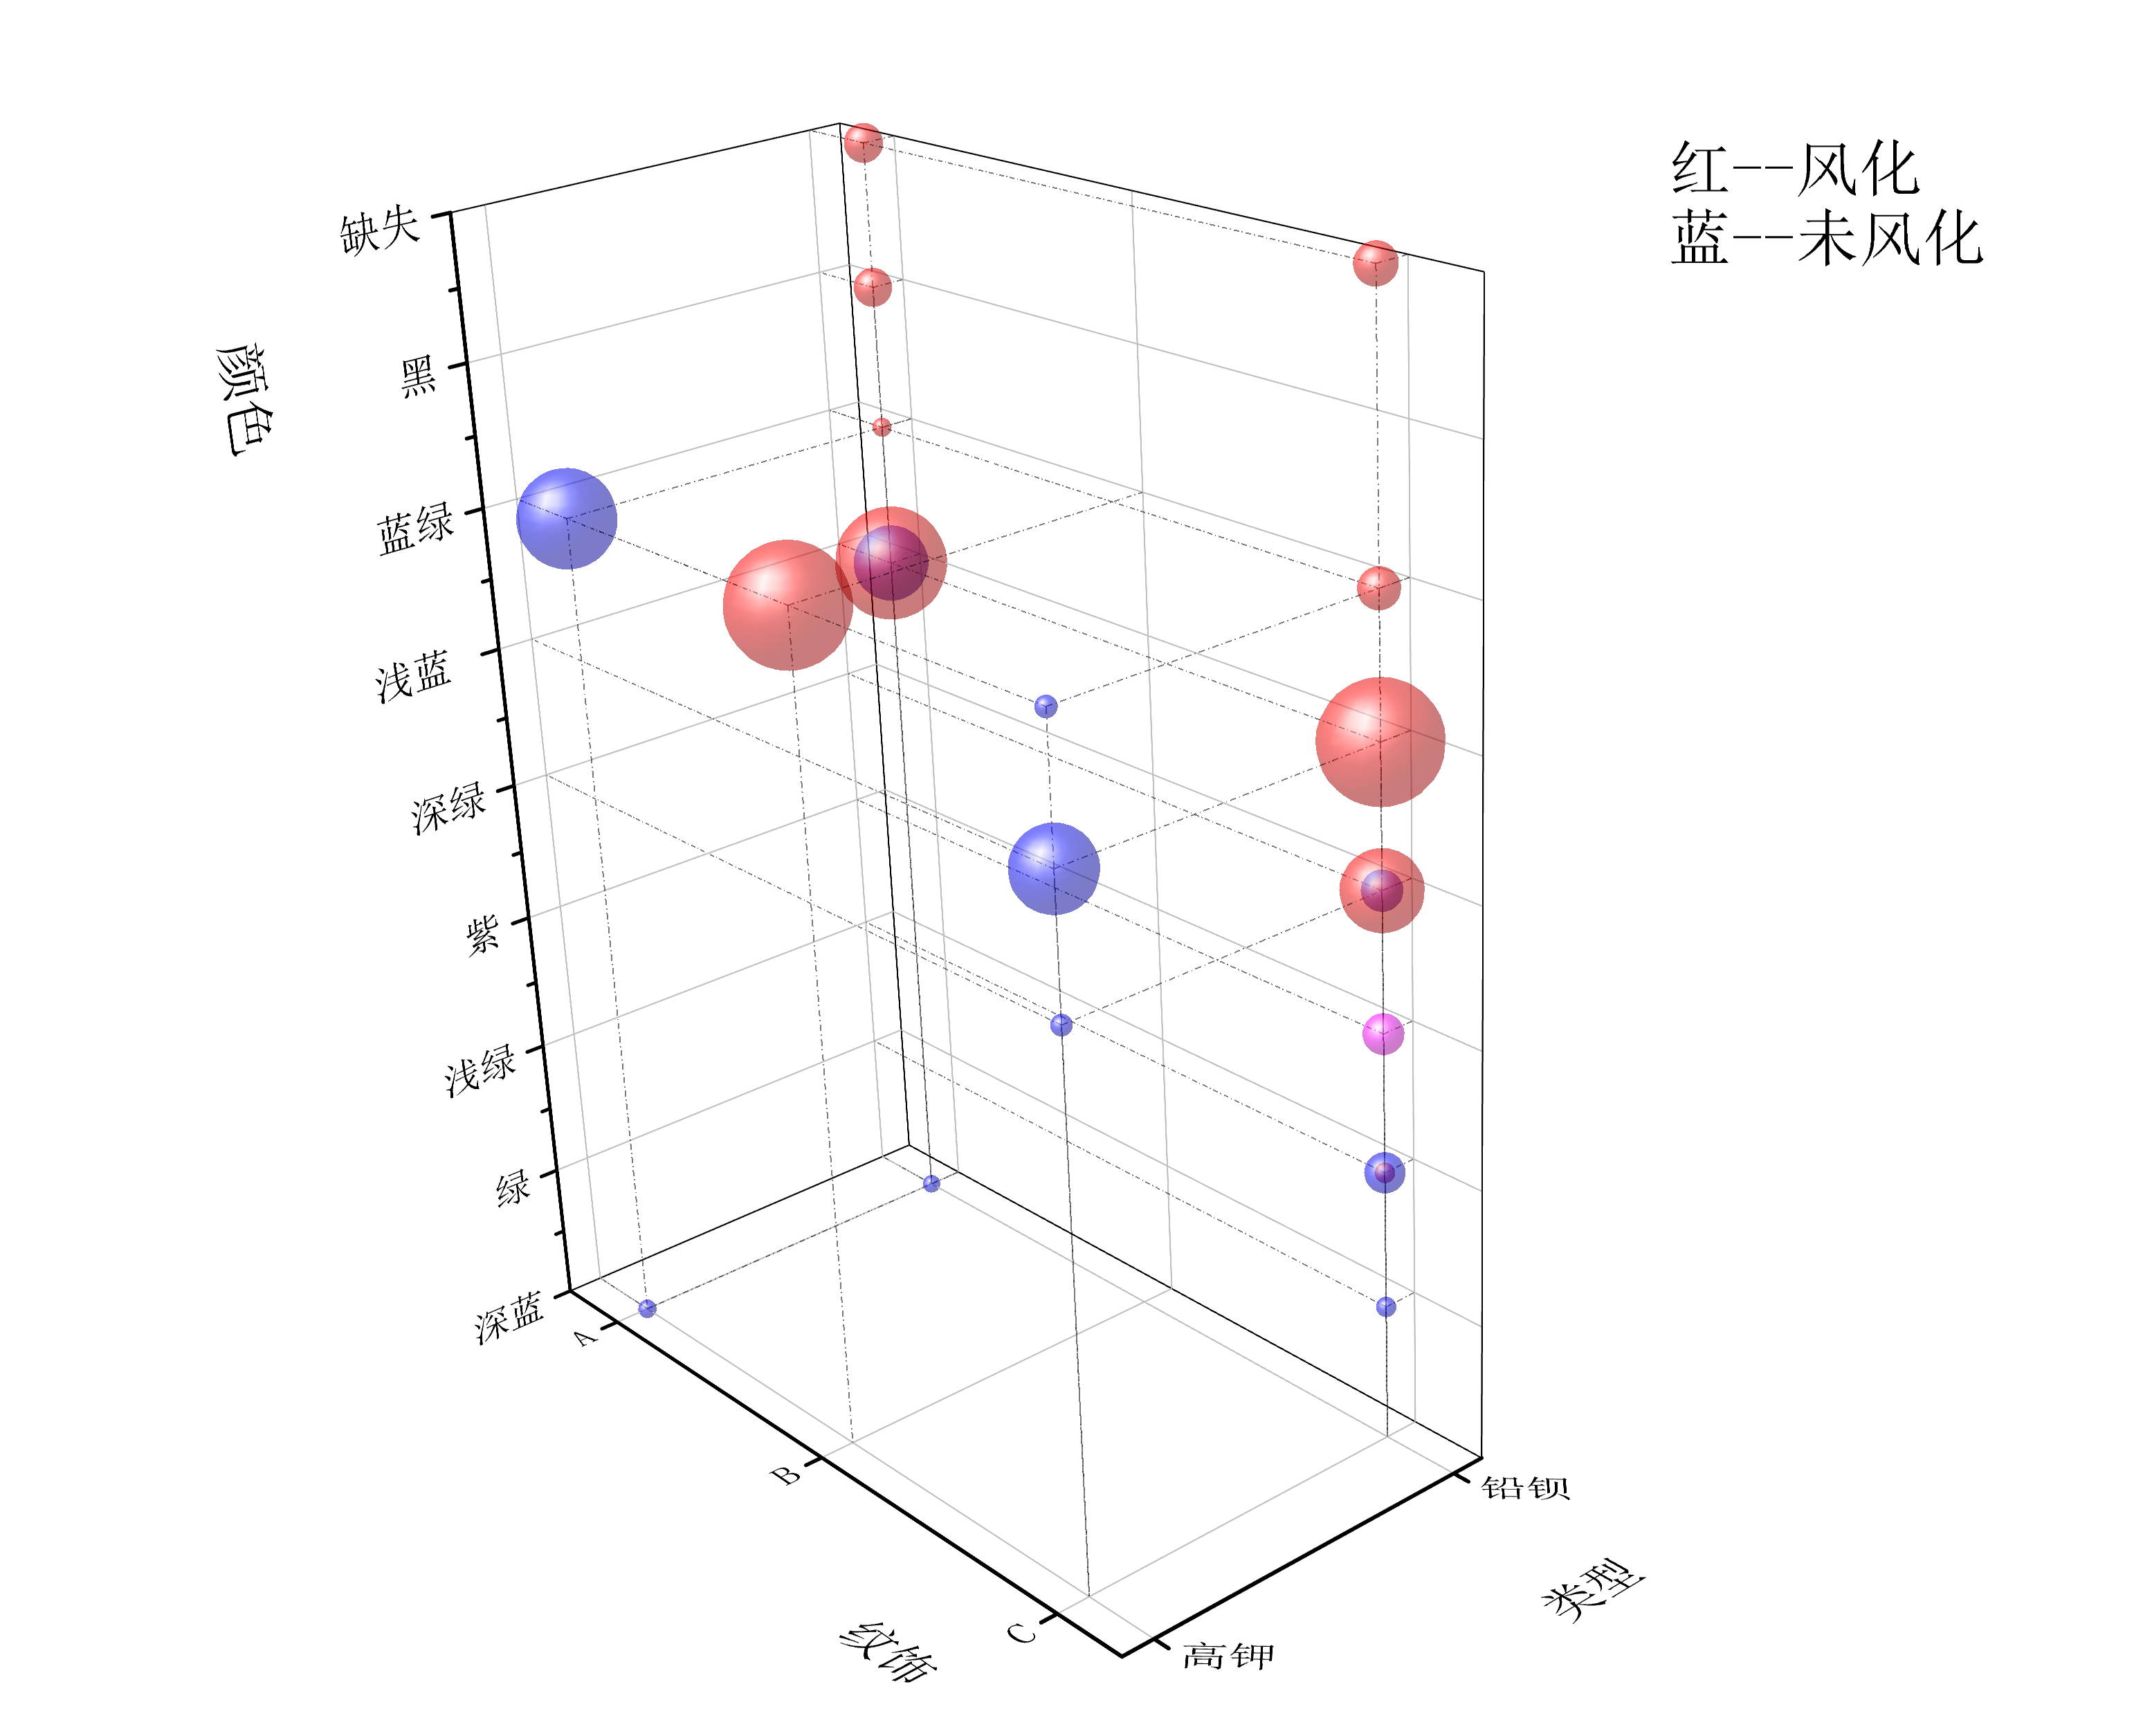
\includegraphics[width=.85\textwidth]{yuansu3d}
	\caption{描述数据整体特征的三维散点气泡图}
	\label{yuansu3d}
\end{figure}


为了得到更加具体的关系特征,对图像进行降维处理,分别得到高钾玻璃和铅钡玻璃的纹饰、颜色与有无分化关系的二维散点图,如图\ref{leixing}所示。

\begin{figure}[!h]
	\centering
	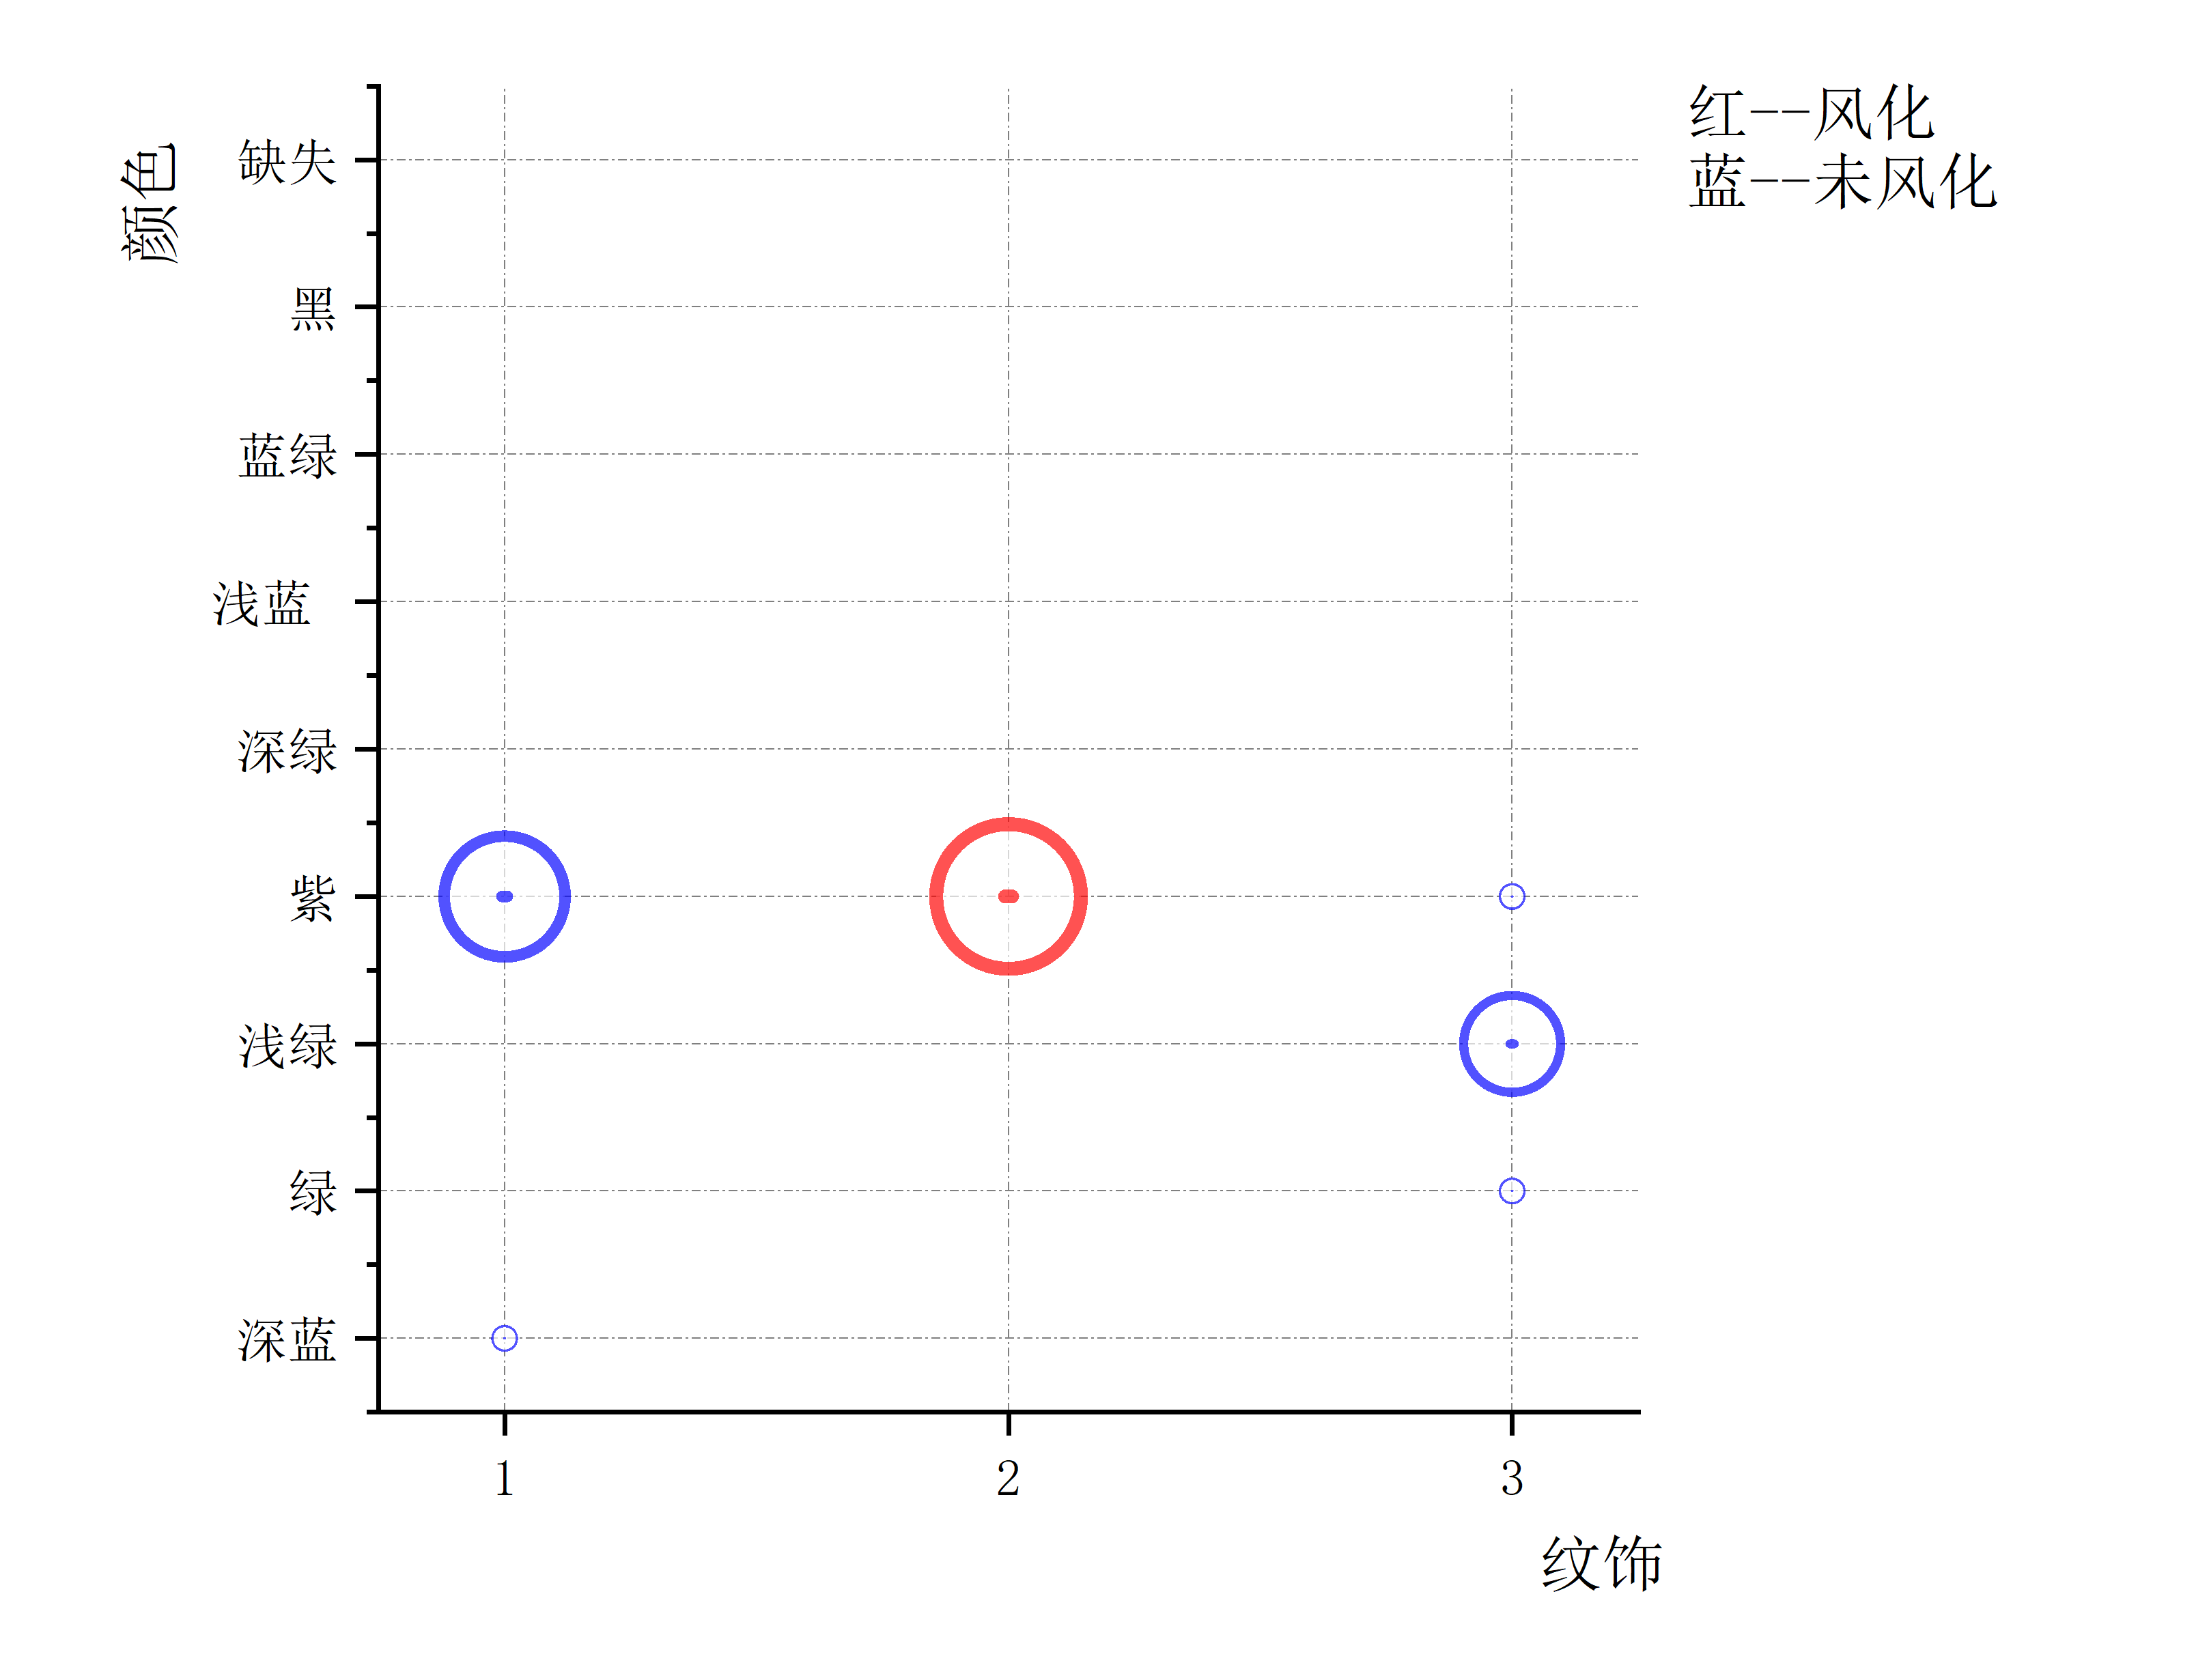
\includegraphics[width=.49\textwidth]{leixing1}
	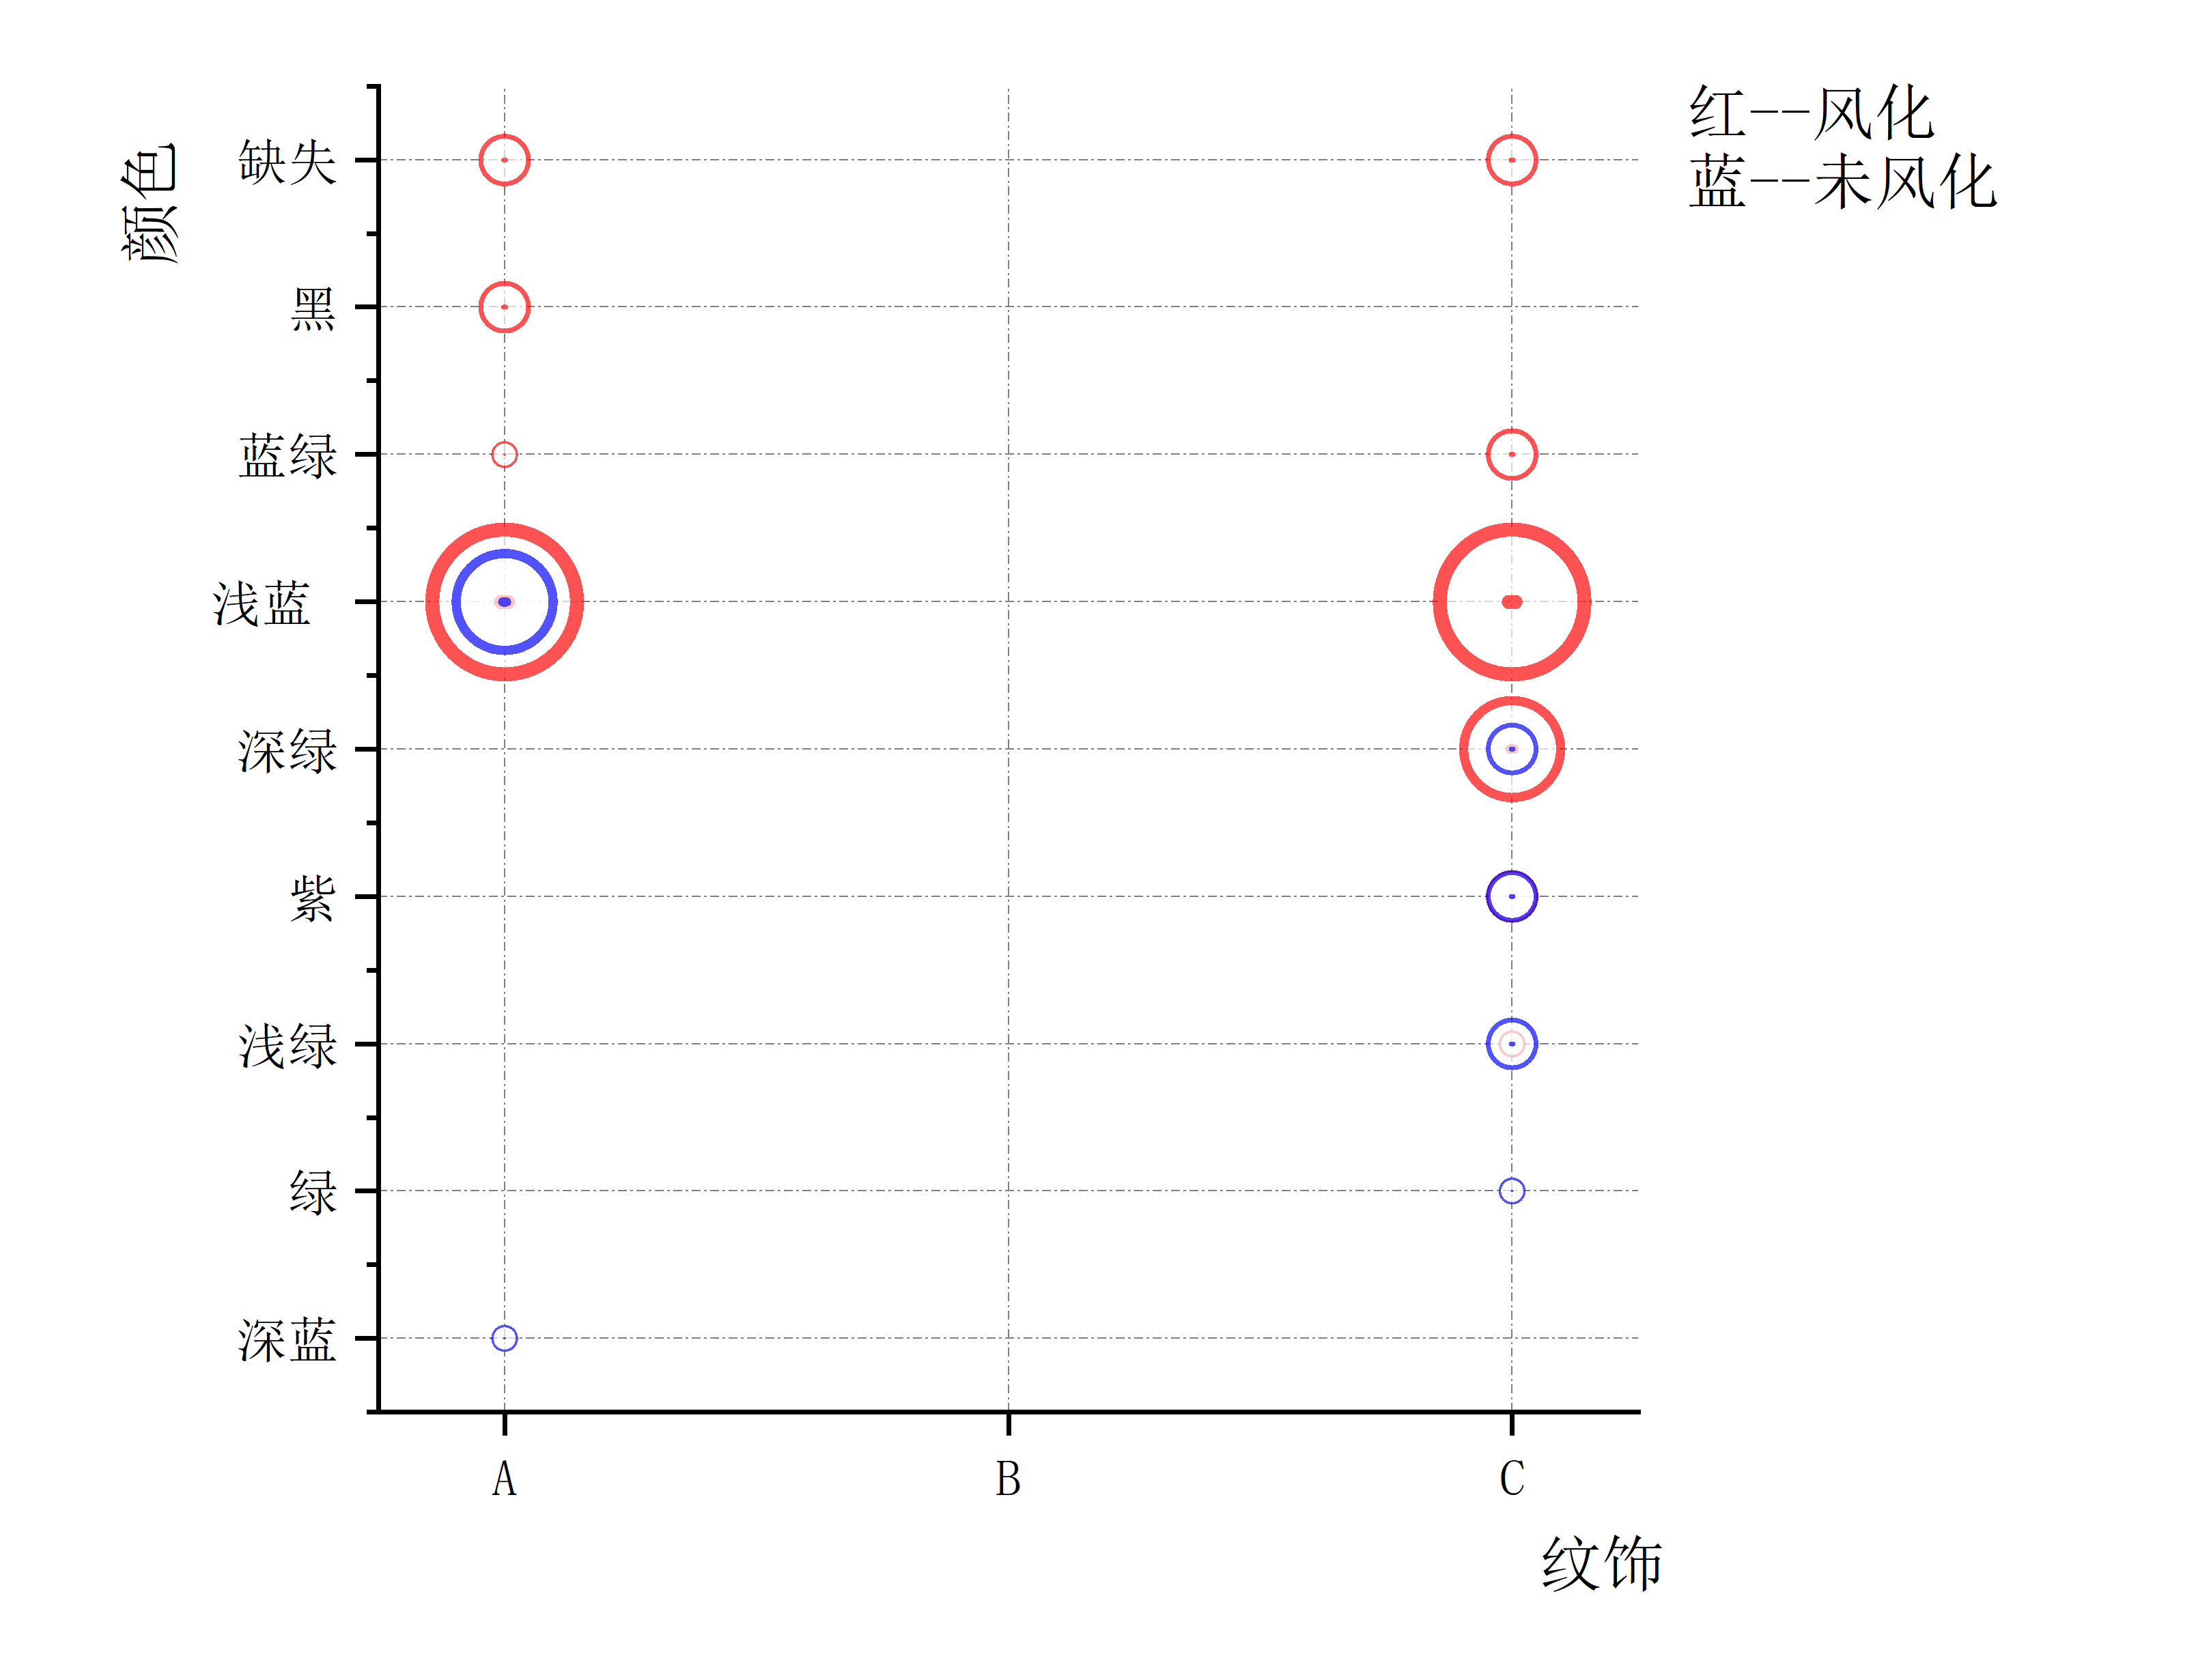
\includegraphics[width=.49\textwidth]{leixing2}
	\caption{描述高钾玻璃(左)和铅钡玻璃(右)数据特征的二维散点图}
	\label{leixing}
\end{figure}


由图,可以得出如下的规律:
\begin{itemize}
	\item 由高钾玻璃的二维图,可以观察到高钾玻璃中B纹饰——紫颜色的种类风化结果表现为风化,且数据样本较多,其他类型的纹饰与颜色均表现为未风化;
	\item 由铅钡玻璃的二维图,可以观察到A纹饰的浅蓝色同时表现出了未风化、风化两种结果,推测当A纹饰的铅钡玻璃介于风化与未风化的过渡地带时,往往呈现出浅蓝色,而A纹饰的其他颜色都具有较好的区分属性,如A纹饰——深蓝色表现为未风化,而A纹饰——蓝绿色/黑色/缺失颜色均表现为风化;
	\item 由铅钡玻璃的二维图,可以观察到C纹饰的深绿色、紫色、浅绿色同时表现出了未风化、风化两种结果,推测当C纹饰的铅钡玻璃介于风化与未风化的过渡地带时,往往呈现出这三种颜色,而C纹饰的其他颜色,如C纹饰——绿色表现为未风化,C纹饰——蓝绿色/缺失颜色均表现为风化。
\end{itemize}


基于上述的规律,本文做出了三个维度数据与风化结果的关系特征的推导:
\begin{itemize}
	\item 玻璃类型会对风化结果产生较显著的影响,铅钡玻璃风化比重比高钾玻璃大
	\item 风化过程中会存在颜色的渐变,这种渐变过程会因玻璃类型和纹饰存在差异,如铅钡玻璃的C纹饰,初始为绿色,经过风化由于化学成分改变逐渐变成浅绿、深绿的过度颜色,最终被完全风化,变成蓝绿色。
\end{itemize}


\subsection{基于Spearman相关系数的按含量比例分类的分类模型}

本文设计了基于Spearman相关系数的按含量比例分类的模型,具体流程如下所示:

首先针对高钾玻璃做具体的流程分析:
\begin{itemize}
	\item Step1: 绘制高钾玻璃风化前后的各个归一化后的化学成分含量的散点图如图\ref{gjfh}所示,观察数据特征。
	
	\begin{figure}[!h]
		\centering
		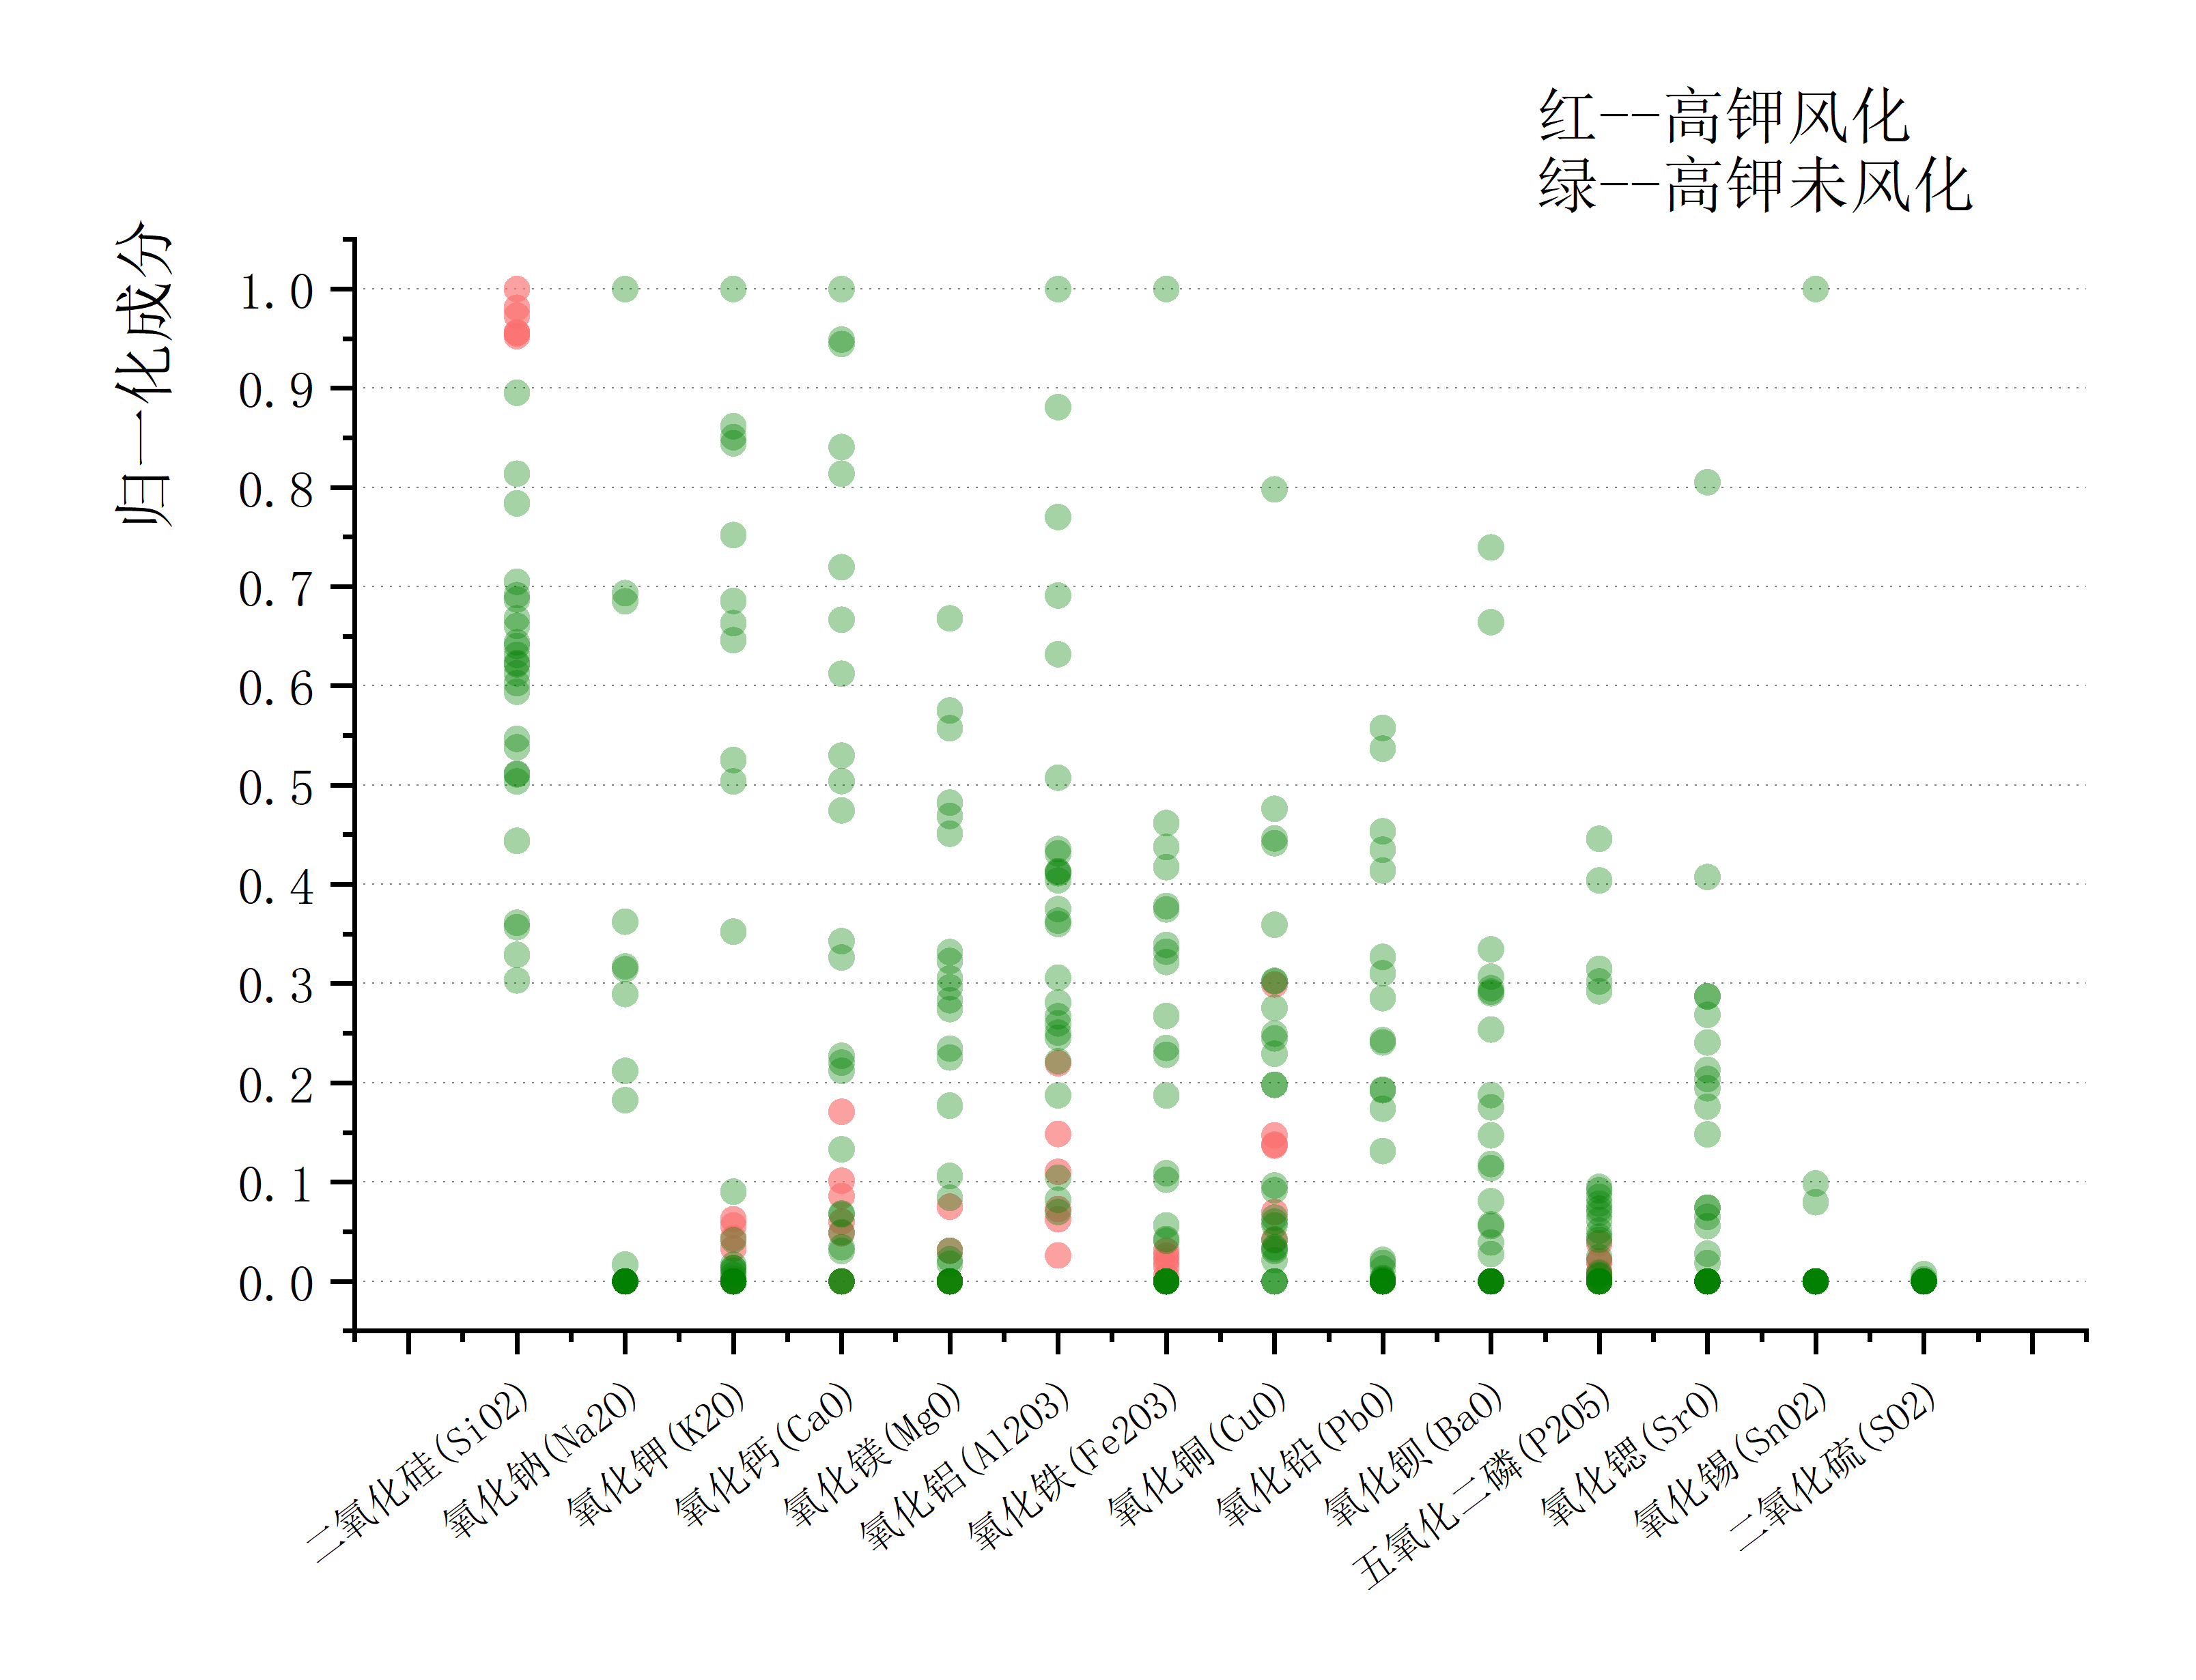
\includegraphics[width=.85\textwidth]{高钾风化与否}
		\caption{高钾玻璃风化前后归一化后成分含量散点图}
		\label{gjfh}
	\end{figure}
	
	由图\ref{gjfh}可以初步得出,高钾玻璃风化前后对部分化学成分含量有较大影响,其中,对$SiO_{2}$的含量有正向影响、对$K_{2}O$、$CaO$、$MgO$、$Al_{2}O_{3}$、$Fe_{2}O_{3}$、$CuO$、$P_{2}O_{5}$的含量有负向影响。
	
	\item Step2: 计算高钾玻璃各个化学成分的Spearman相关系数。
	
	 定义:X和Y为两组数据,其斯皮尔曼(等级)相关系数为:
	 \[
	 r_{s}=1-\frac{6 \sum_{i=1}^{n} d_{i}^{2}}{n\left(n^{2}-1\right)}
	 \]
	
	 其中,di为Xi和Yi之间的等级差。
	
	若某两种Spearman相关性较大,则可以推测在风化前后这两种化学成分极可能存在某种化学转换关系,结合步骤1,由于众多成分中只有$SiO_{2}$含量明显减少,故主要探究$SiO_{2}$与其他化学成分含量的Spearman系数,将各成分间的Spearman相关系数按颜色划分,得到热力图如图\ref{Spearman}所示。
	
	\begin{figure}[!h]
		\centering
		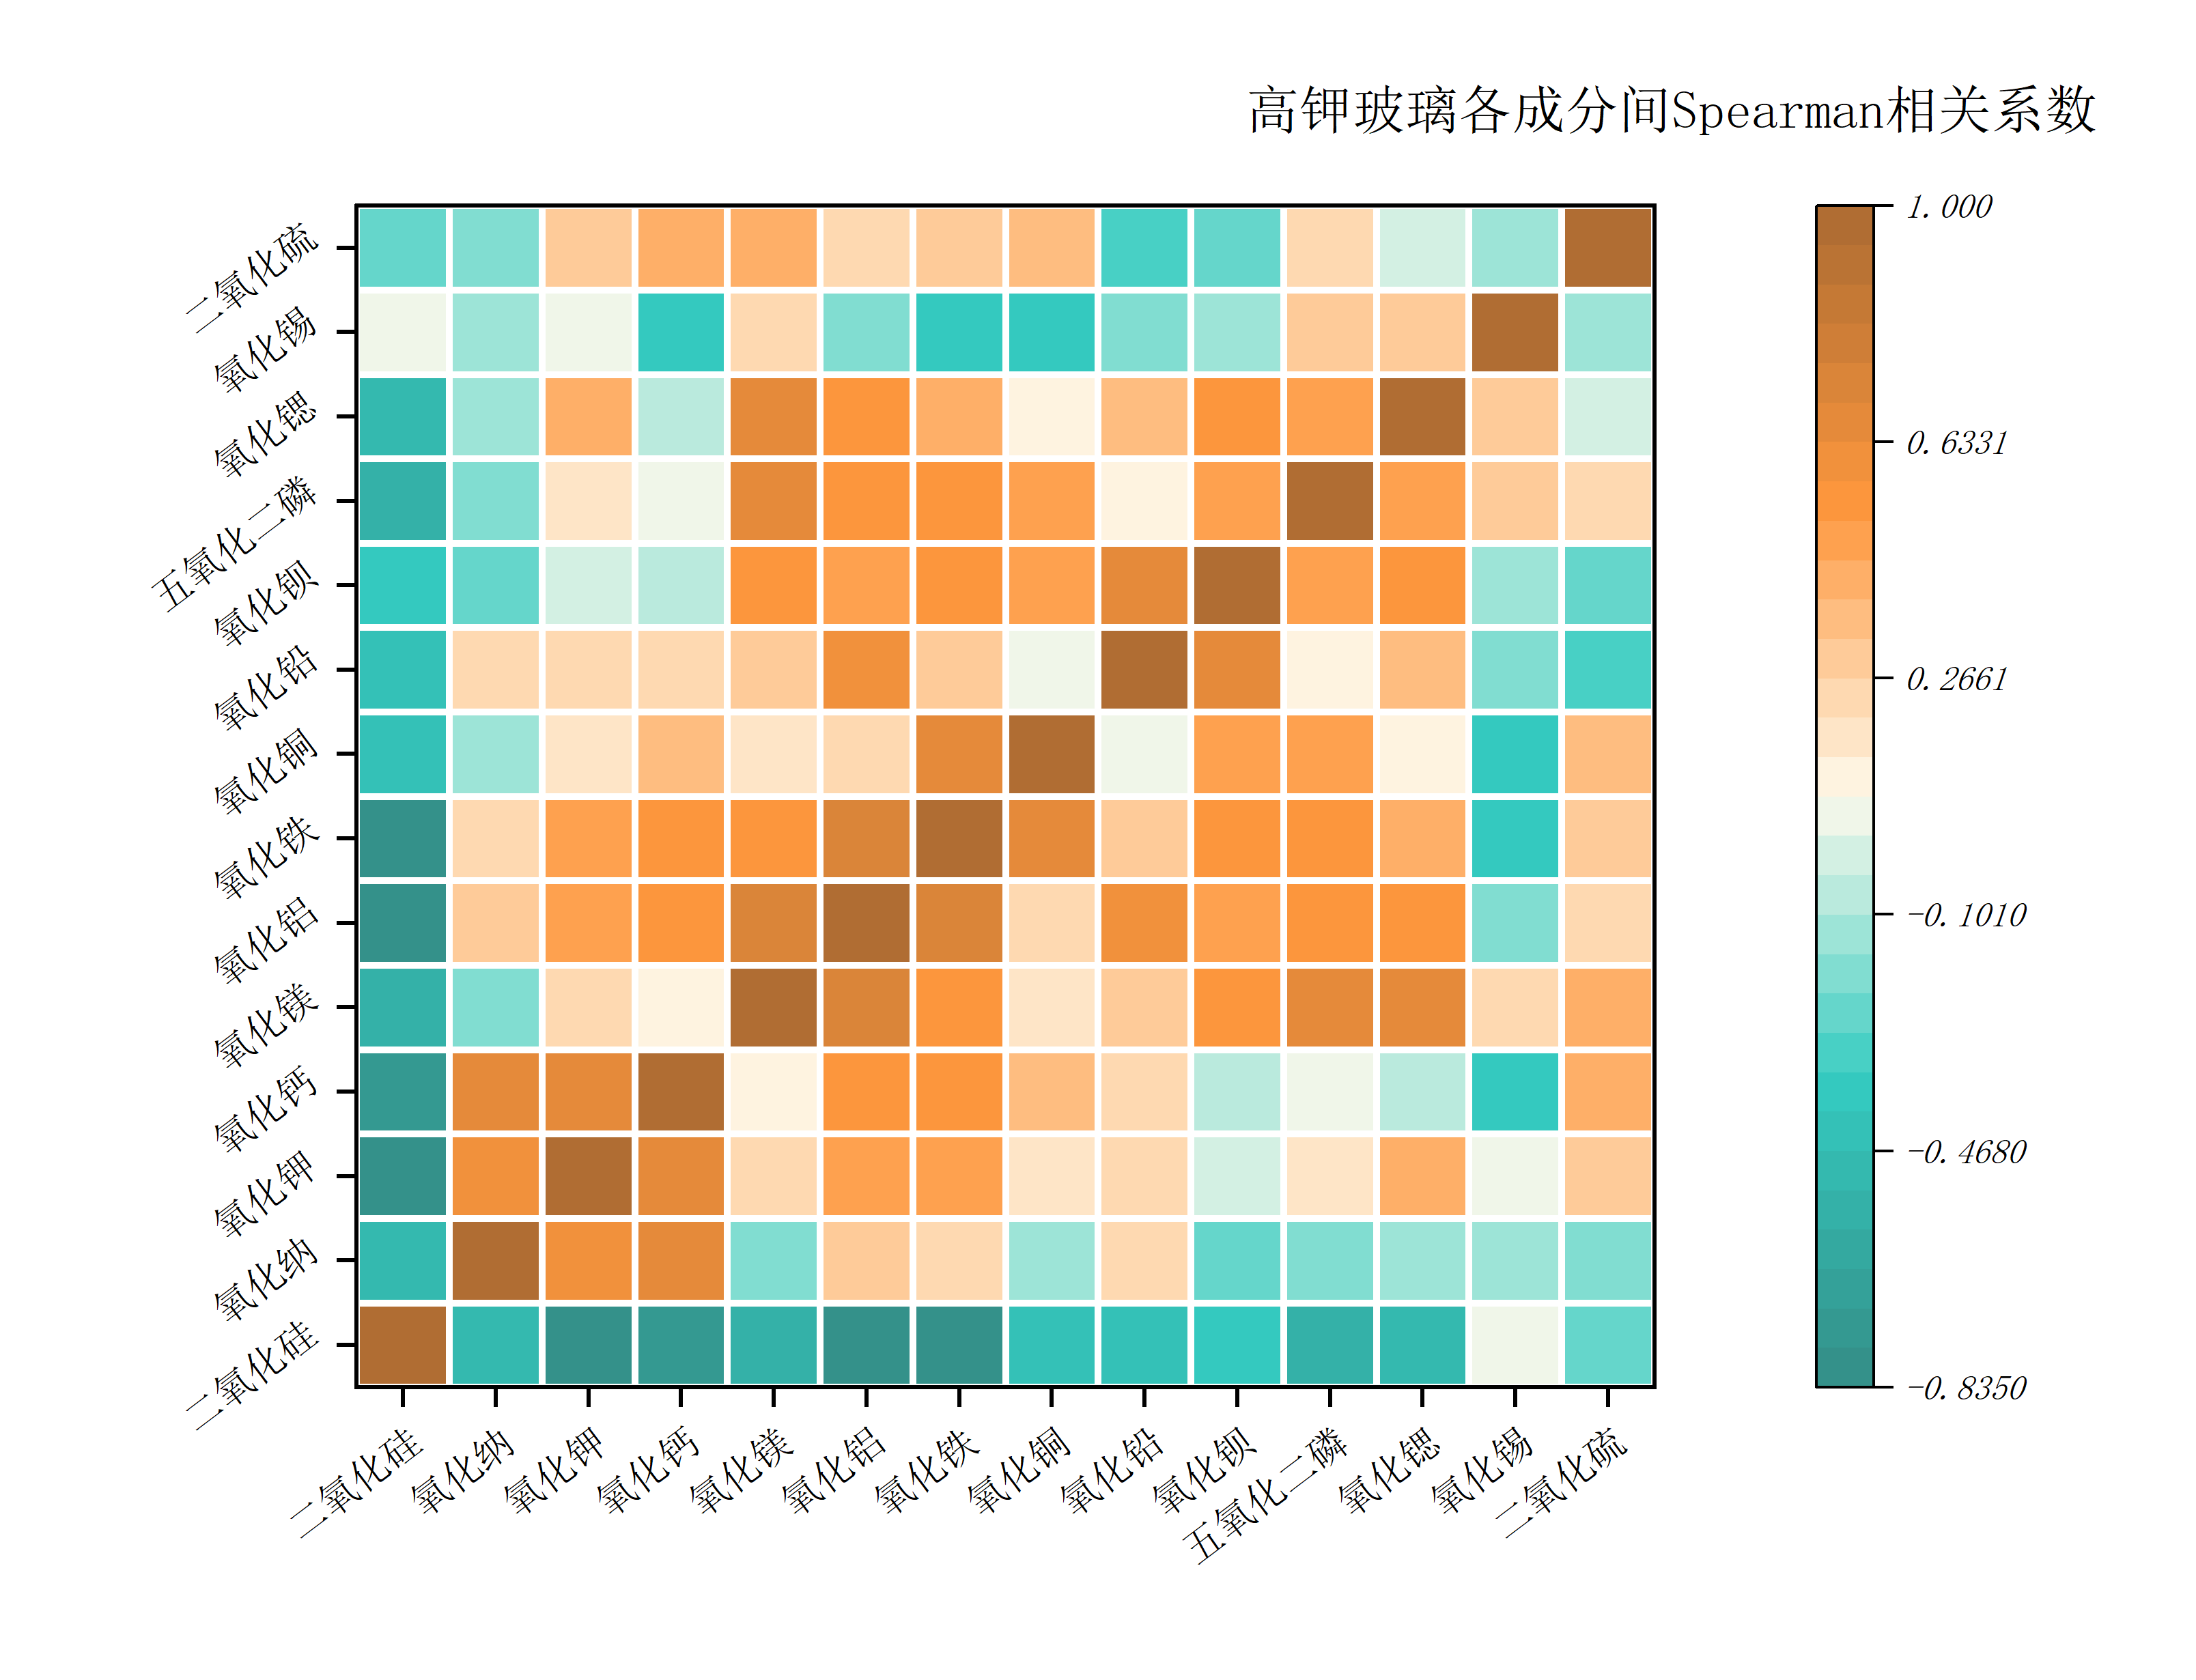
\includegraphics[width=.85\textwidth]{Spearman相关系数}
		\caption{高钾玻璃各成分间的Spearman相关系数热力图}
		\label{Spearman}
	\end{figure}

	
以Spearman相关系数0.6为分界,选出与$SiO_{2}$相关性最强的五个化学成分,分别为:$K_{2}O$、$CaO$、$MgO$、$Al_{2}O_{3}$、$Fe_{2}O_{3}$,此结果与步骤一的结果得到了相互印证。
	
	
	\item Step3:以化学成分含量的比例作为是否风化的依据。
	
	 基于上述分析,构造$SiO_{2}$与其他五个化学成分的比例关系$p_{1}$,$p_{1}$公式如下所示: $$p_{1}=\frac{n(SiO_{2})}{n(K_{2}O)+n(CaO)+n(MgO)+n(Al_{2}O_{3})+n(Fe_{2}O_{3})}$$ 各个高钾玻璃的文物样品的$p_{1}$如表\ref{gjp}所示,由于篇幅关系,仅展示6个风化样品与6个未风化样品的$p_{1}$值,完整表格见附录n。
	
	
	\begin{table}[!h]
		\centering
		\caption{高钾玻璃样品的$p_{1}$值}
		\label{gjp}
		\begin{tabular}{@{}ccccccccc@{}}
			\toprule
			\textbf{类型} & \textbf{表面风化} & \textbf{\begin{tabular}[c]{@{}c@{}}二氧化硅\\ (SiO2)\end{tabular}} & \textbf{\begin{tabular}[c]{@{}c@{}}氧化钾\\ (K2O)\end{tabular}} & \textbf{\begin{tabular}[c]{@{}c@{}}氧化钙\\ (CaO)\end{tabular}} & \textbf{\begin{tabular}[c]{@{}c@{}}氧化镁\\ (MgO)\end{tabular}} & \textbf{\begin{tabular}[c]{@{}c@{}}氧化铝\\ (Al2O3)\end{tabular}} & \textbf{\begin{tabular}[c]{@{}c@{}}氧化铁\\ (Fe2O3)\end{tabular}} & \textbf{\begin{tabular}[c]{@{}c@{}}高钾的比例\\ (区分风化)\end{tabular}} \\ \midrule
			高钾          & 风化            & 96.77                                                          & 0.92                                                         & 0.21                                                         & 0.00                                                         & 0.81                                                           & 0.26                                                           & 43.99                                                           \\
			高钾          & 风化            & 95.02                                                          & 0.59                                                         & 0.62                                                         & 0.00                                                         & 1.32                                                           & 0.32                                                           & 33.34                                                           \\
			高钾          & 风化            & 92.63                                                          & 0.00                                                         & 1.07                                                         & 0.00                                                         & 1.98                                                           & 0.17                                                           & 28.77                                                           \\
			高钾          & 风化            & 94.29                                                          & 1.01                                                         & 0.72                                                         & 0.00                                                         & 1.46                                                           & 0.29                                                           & 27.09                                                           \\
			高钾          & 风化            & 92.72                                                          & 0.00                                                         & 0.94                                                         & 0.54                                                         & 2.51                                                           & 0.20                                                           & 22.13                                                           \\
			高钾          & 风化            & 92.35                                                          & 0.74                                                         & 1.66                                                         & 0.64                                                         & 3.50                                                           & 0.35                                                           & 13.40                                                           \\
			高钾          & 无风化           & 60.71                                                          & 5.71                                                         & 0.00                                                         & 0.85                                                         & 0.00                                                           & 1.04                                                           & 7.99                                                            \\
			高钾          & 无风化           & 87.05                                                          & 5.19                                                         & 2.01                                                         & 0.00                                                         & 4.06                                                           & 0.00                                                           & 7.73                                                            \\
			高钾          & 无风化           & 79.46                                                          & 9.42                                                         & 0.00                                                         & 1.53                                                         & 3.05                                                           & 0.00                                                           & 5.68                                                            \\
			高钾          & 无风化           & 76.68                                                          & 0.00                                                         & 4.71                                                         & 1.22                                                         & 6.19                                                           & 2.37                                                           & 5.29                                                            \\
			高钾          & 无风化           & 61.87                                                          & 7.44                                                         & 0.00                                                         & 1.02                                                         & 3.15                                                           & 1.04                                                           & 4.89                                                            \\ \bottomrule
		\end{tabular}
	\end{table}
	
	
	依照表格信息,可以选取$p_{1}=10.7$作为区分高钾玻璃风化与否的依据。
	
	\item Step4:总结统计规律。
	
	
	 当高钾玻璃中的$p_{1}=\frac{n(SiO_{2})}{n(K_{2}O)+n(CaO)+n(MgO)+n(Al_{2}O_{3})+n(Fe_{2}O_{3})}$大于10.7时,高钾玻璃出现风化,小于10.7时,高钾玻璃不风化。
	
\end{itemize}


接着对铅钡玻璃进行分析,铅钡玻璃的分析流程与高钾玻璃类似,首先得出铅钡玻璃的风化前后化学成分含量的散点图,如图\ref{qbfh}所示


\begin{figure}[!h]
	\centering
	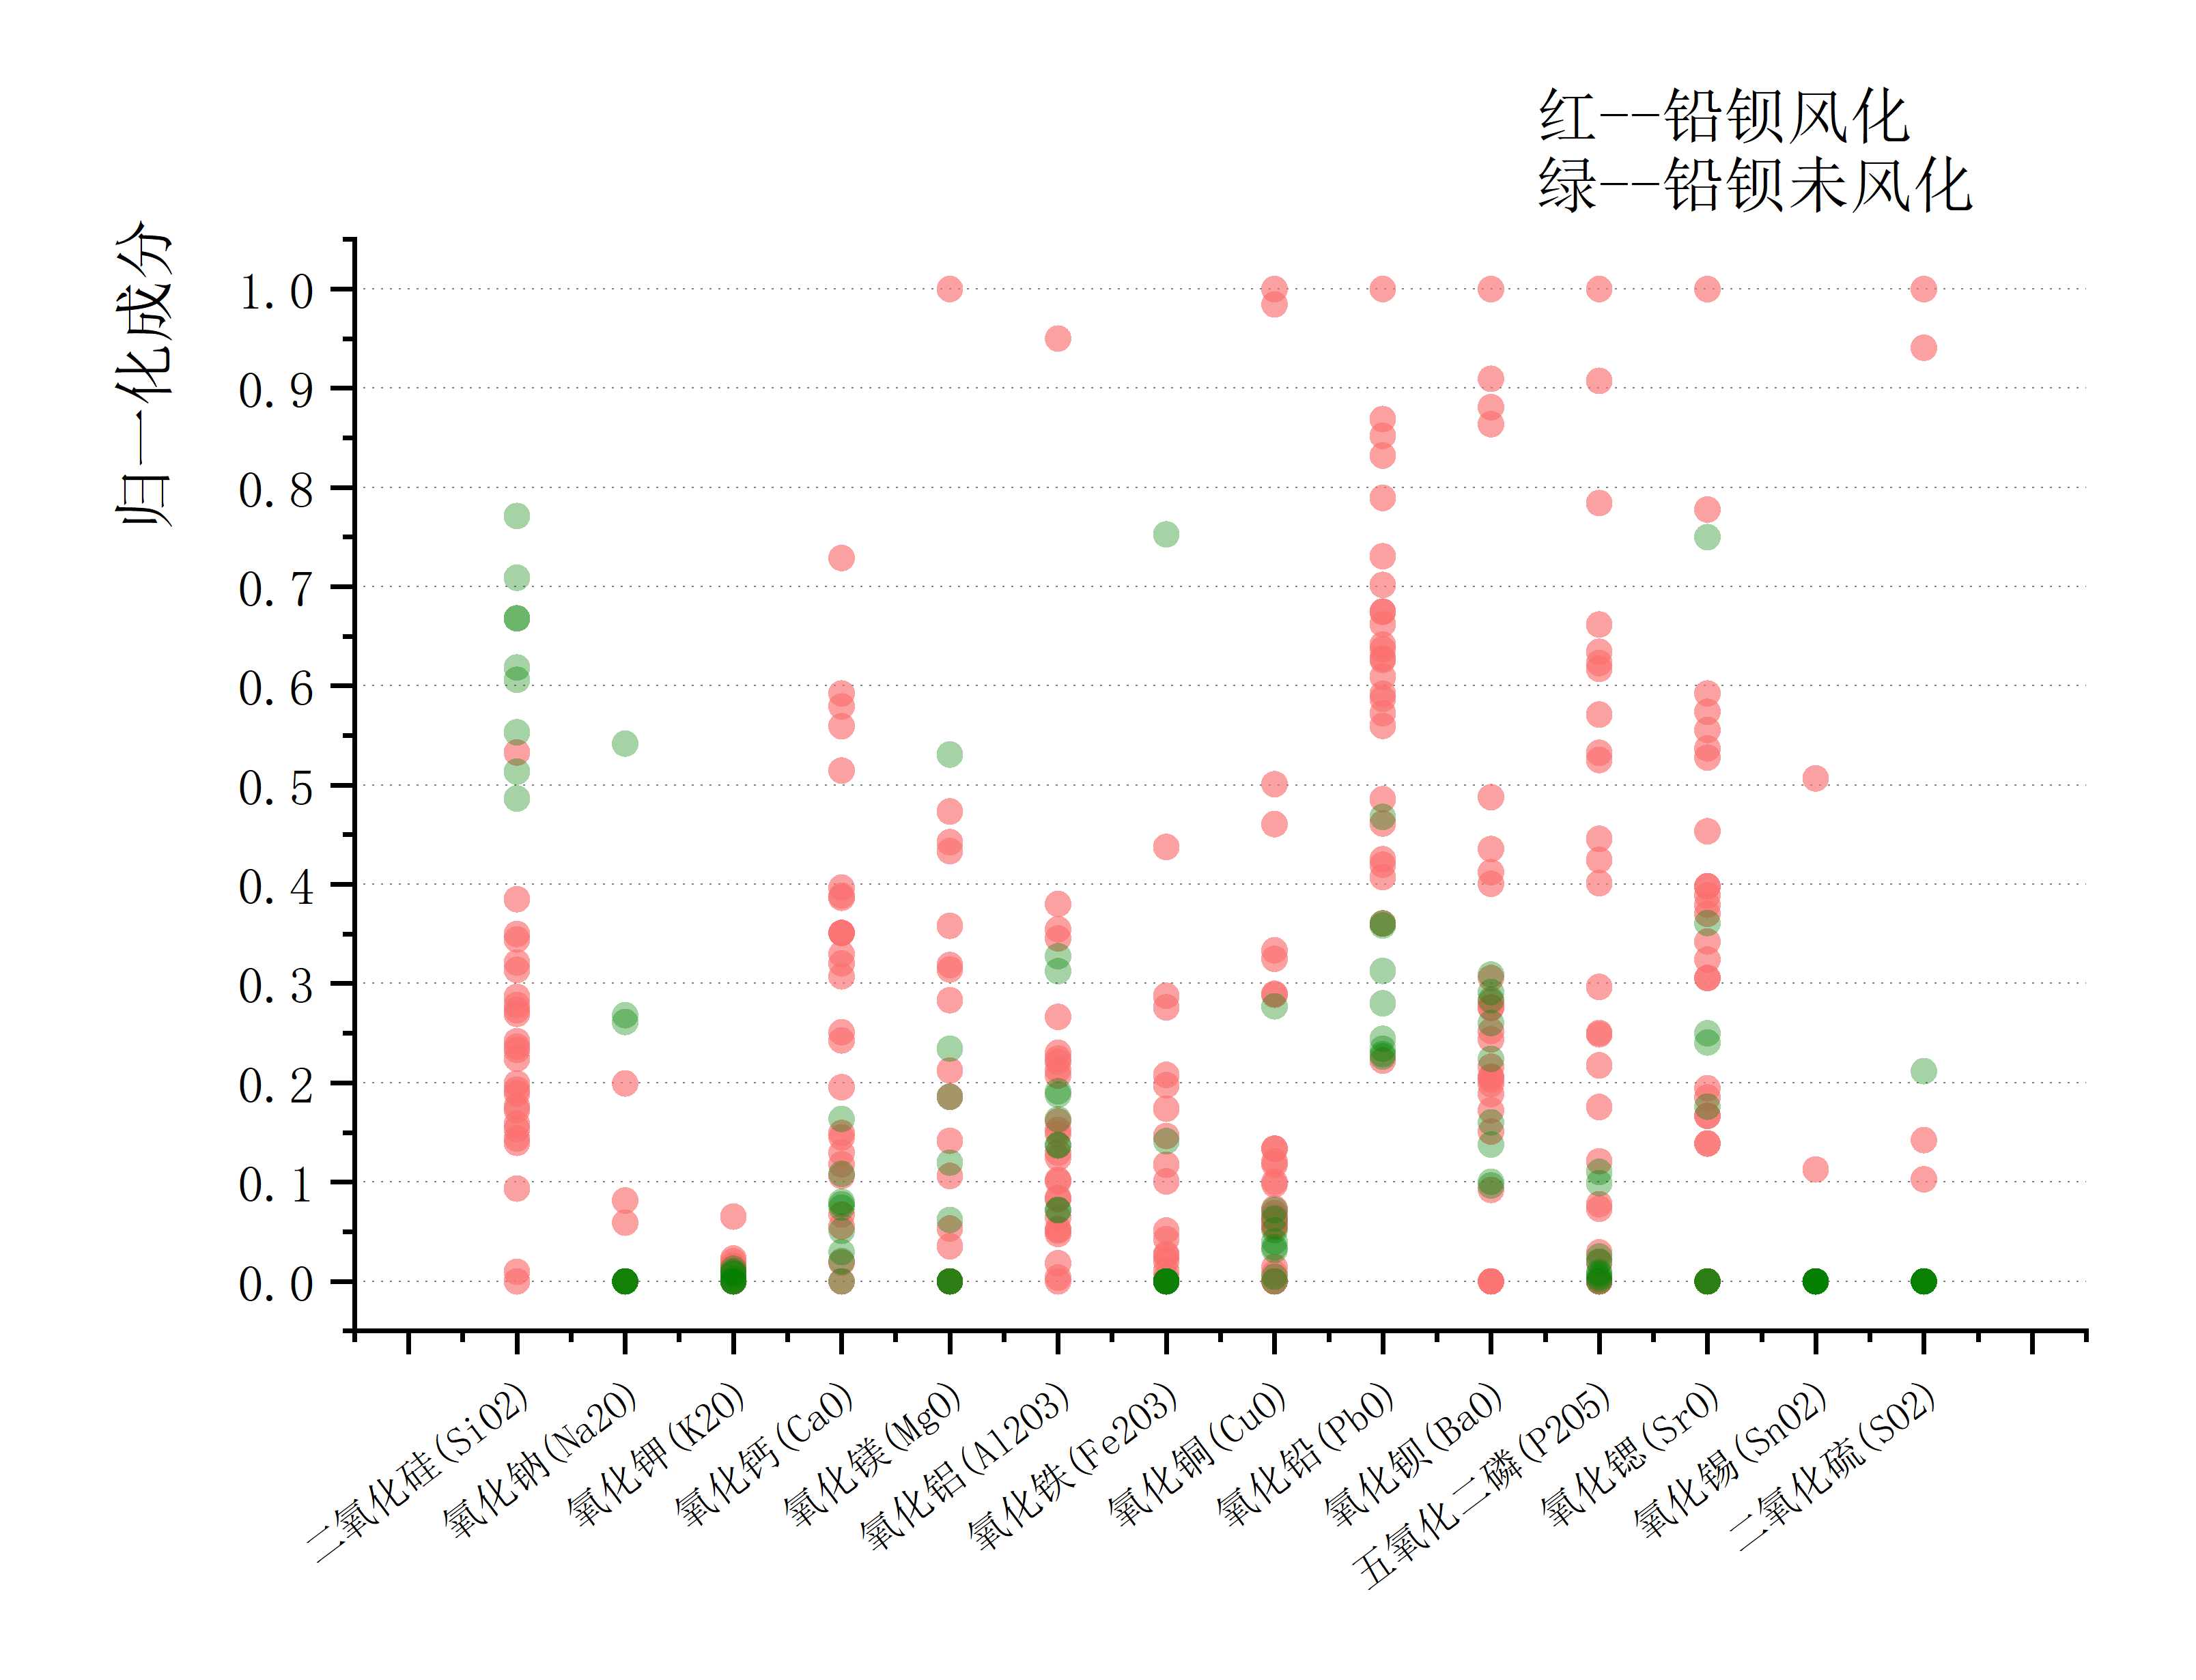
\includegraphics[width=.85\textwidth]{铅钡风化与否}
	\caption{铅钡玻璃风化前后归一化后成分含量散点图}
	\label{qbfh}
\end{figure}


从图中除了能分析出风化后$SiO_{2}$含量减少之外,较难分析铅钡玻璃中风化前后化学成分的变化,故需要求解Spearman相关系数进行进一步观察,可视化Spearman相关系数热力图如图\ref{Spearman2}所示。


\begin{figure}[!h]
	\centering
	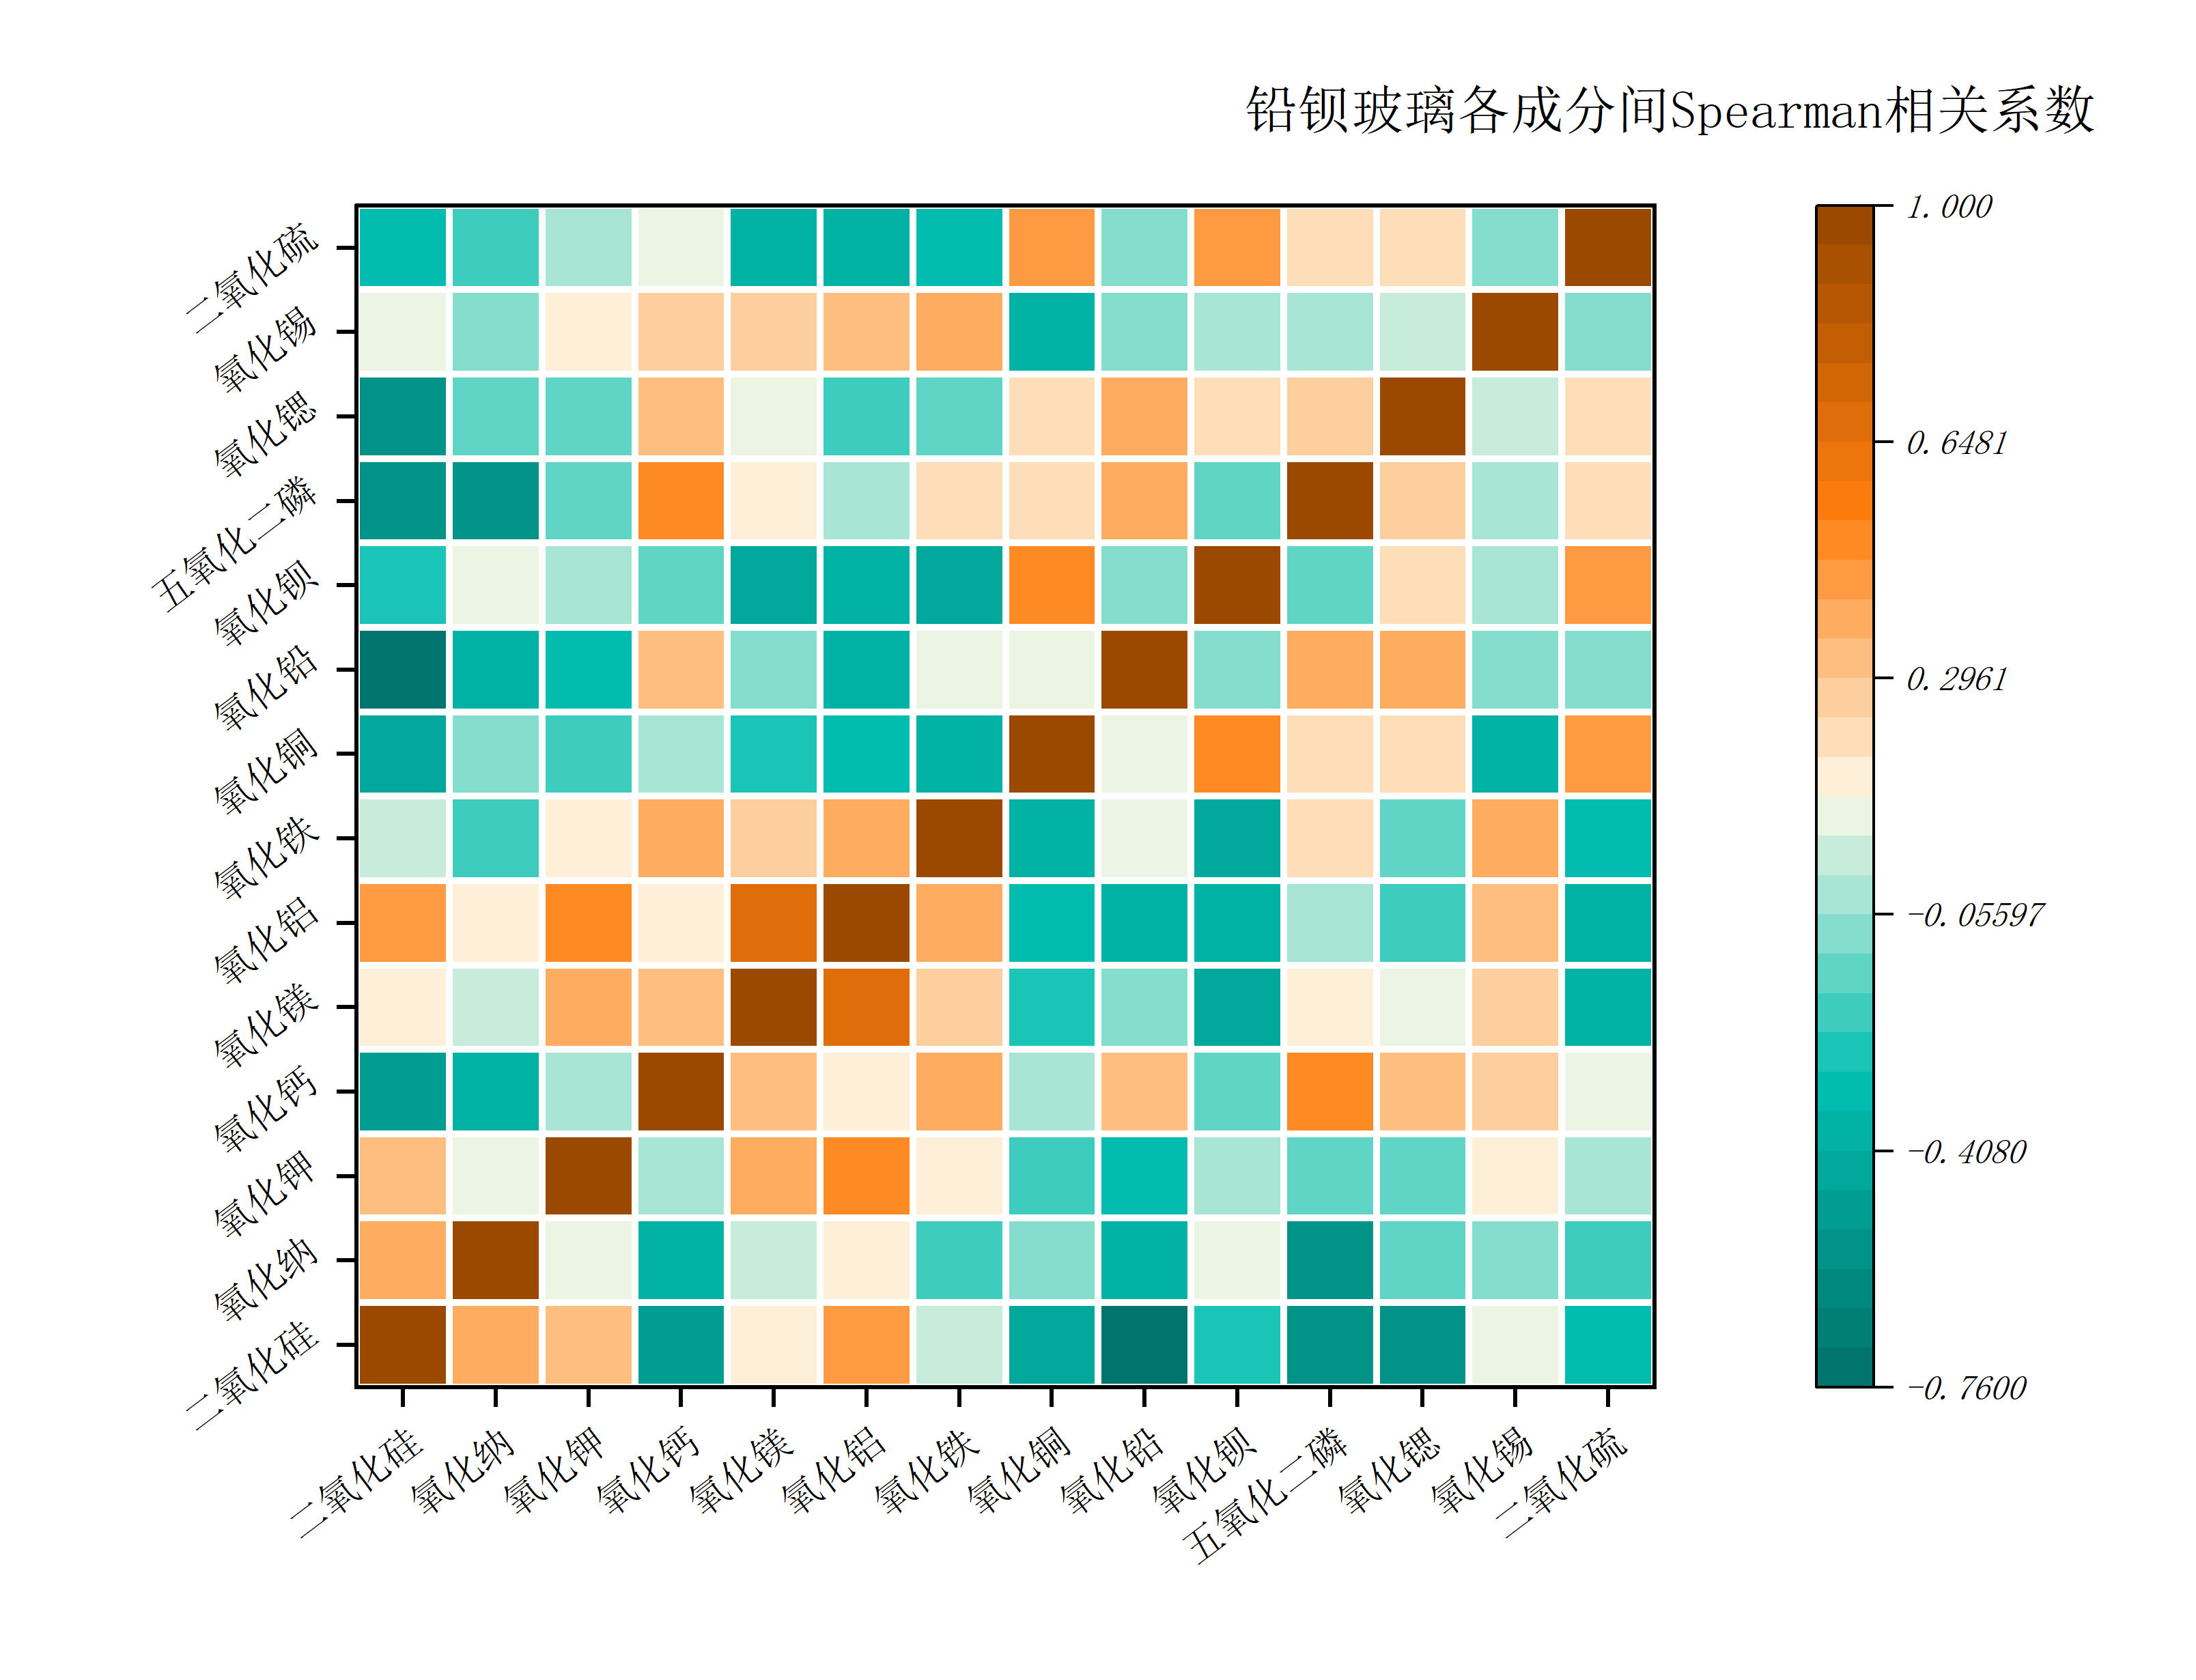
\includegraphics[width=.85\textwidth]{Spearman相关系数2}
	\caption{铅钡玻璃各成分间的Spearman相关系数热力图}
	\label{Spearman2}
\end{figure}


\newpage
%参考文献
\begin{thebibliography}{9}%宽度9
	\bibitem[1]{test} 参考文献
\end{thebibliography}



\newpage
%附录
\begin{appendices}
	

	\section{附录}

\begin{python}
import math

def hix(x):
if x > 0:
return 1+1=2
else:
return 0

\end{python}




\end{appendices}





\end{document} 